\documentclass[12pt,a4paper,titlepage]{article}
%va sempre messo article per "program documentation"
\usepackage[italian]{babel}
\usepackage[T1]{fontenc}
\usepackage[latin1]{inputenc}
\usepackage{titlesec}
\usepackage[hidelinks]{hyperref}
\usepackage[a4paper,top=2cm,bottom=2cm,left=1cm,right=1cm]{geometry}
\usepackage{soulutf8,color}
\usepackage{multirow}
\usepackage{lscape}
\usepackage{graphicx}
\usepackage{eurosym} %per il simbolo dell' \euro


\usepackage{emptypage} 
% pagine vuote senza testatina e piede di pagina

%\usepackage{hyperref} 
% collegamenti ipertestuali

\usepackage{fancyhdr}
% pacchetto per intestazione e pie pagina

\pagestyle{fancy}
\usepackage{lastpage}


% \textsubscript{g} per indicare termini nel glossario

% \\ indica interruzione di riga

% compilate 2 volte per documenti con indice

% {\em qui testo in corsivo}
% {\bfseries qui testo in grossetto}

%LISTE NUMERATE
%\begin{enumerate}
%\item primo
%\item secondo
%\item terzo
%\end{enumerate}

%LISTE PUNTATE
%\begin{itemize}
%\item primo
%\item secondo
%\item \dots
%\end{itemize}

%TABELLA
%\begin{tabular}{|c|c|c|}
%indica una tabella con 3 colonne e pos. testo centrale. La barra verticale ( | ) indica che vi è una linea divisoria verticale tra le celle.
%\hline	linea separatrice orizzontale
%testo1& testo2& testo3\\
% & segna la fine del testo nella cella, \\ indica il fine della riga 

\newcommand{\minitab}[2][1]{\begin{tabular}#1 #2\end{tabular}}

%GRAFICI
%\begin{figure}
%\includegraphics{filegrafico}
%comando per includere le immagini (controllare i formati)
%\caption{didascalia}
%\label{nome}
%\end{figure}

%----------------------------------------------------------- INIZIO TEMPLATE TITOLO

\usepackage{xcolor} % Importa i colori per la prima pagina
\usepackage{fix-cm} % Permette l'incremento del font oltre misura

\newcommand{\HRule}[1]{\hfill \rule{0.2\linewidth}{#1}} % Horizontal rule at the bottom of the page, adjust width here

\definecolor{grey}{rgb}{0.9,0.9,0.9} % Colore del box del titolo

\begin{document}
	
	\thispagestyle{empty} % Toglie il numero della pagina nella prima pagina
	
	%----------------------------------------------------------------------------------------
	%	TITLE SECTION
	%----------------------------------------------------------------------------------------
	
	\colorbox{grey}{
		\parbox[t]{1.0\linewidth}{
			\centering \fontsize{50pt}{80pt}\selectfont % Il primo è la grandezza del font, il secondo lo spazio lasciato
			\vspace*{0.7cm} % Spazio dall'inizio del box al titolo
			
			\raggedleft
			
\includegraphics[width=0.7\linewidth]{../../LogoSWEgGroupSFONDOVUOTO}
			
			\hfill Piano di Progetto \\
			
			\vspace*{0.7cm} % Spazio dalla fine del testo alla fine del box
		}
	}
	
	%----------------------------------------------------------------------------------------
	
	\vfill % Spazio dalla fine del box alle altre informazioni
	
	%----------------------------------------------------------------------------------------
	%	Informazioni sul documento
	%----------------------------------------------------------------------------------------
	
	{\centering \large 
		\hfill \textbf{Versione} 1.1.0 \\		
		\hfill \textbf{Data di Rilascio} 28/02/2017 \\ 
		\hfill \textbf{Redazione} Sebastiano Marchesini \\
		\hfill Piergiorgio Danieli \\
		\hfill \textbf{Verifica} Pietro Lonardi \\
		\hfill \textbf{Validazione} Alberto Gelmi \\
		\hfill \textbf{Responsabile} Sebastiano Marchesini \\
		\hfill \textbf{Uso} Interno \\
		\hfill \textbf{Destinato} SWEg Group \\ 
		
		\HRule{1pt}
		
		\textbf{Sommario} \\
		Questo documento ha l'obiettivo di misurare l'efficienza e pianificare i processi del progetto.
		
	} % Linea orizzontale di estetica
	
	
	%----------------------------------------------------------------------------------------
	
	\clearpage % Parta bianca finale della pagina
	
	%----------------------------------------------------------- FINE TEMPLATE TITOLO
	
	\lhead{
\includegraphics[width=0.2\linewidth]{../../LogoSWEgGroup}}
	\chead{}
	\lfoot{Piano Di Progetto}
	\cfoot{}
	\rfoot{\thepage\ di \pageref{LastPage}} %compilare due volte per avere il numero di pagine totali
	\renewcommand{\headrulewidth}{0.2pt}
	\renewcommand{\footrulewidth}{0.2pt}
	
	\rhead{Registro Modifiche}
	\section{Registro Modifiche}
	\small %rippicciolisce il testo
	{\renewcommand\arraystretch{1.2} %aumenta l'altezza di ogni riga
		\begin{tabular}{|l|c|c|c|}
			\hline
			{\textbf{Ver.}}&{\textbf{Modifica}}&{\textbf{Nome}}&{\textbf{Data}}\\
			\hline
			1.1.0 & Verifica & Lonardi Pietro & 22/02/2017  \\
			\hline
			1.0.9 & \minitab[c]{Inserimento e calcolo dei capitoli\\ : Distribuzione del Lavoro} & Sebastiano Marchesini & 31/01/2017  \\
			\hline
			1.0.8 & \minitab[c]{Inserimento delle WBS e \\ spiegazione di cosa sono e cosa servono capitolo} & Sebastiano Marchesini & 30/01/2017 \\
			\hline
			1.0.7 & \minitab[c]{Motivazione del consultivo di periodo\\ non conforme alla progettazione} & Sebastiano Marchesini & 30/01/2017 \\
			\hline
			1.0.6 & \minitab[c]{Approfondimento e correzione del Capitolo 4 \\ Cambio illustrazione e approfondimento} & Sebastiano Marchesini & 28/01/2017 \\
			\hline
			1.0.5 & \minitab[c]{Approfondimento e correzione Capitolo 3\\ Attualizzazione situazione corrente} & Sebastiano Marchesini & 27/01/2017 \\ 
			\hline
			1.0.4 & \minitab[c]{Tolte duplicazioni nel Capitolo 3 presenti \\ già nei Riferimenti Narmativi} & Sebastiano Marchesini & 26/01/2017 \\
			\hline
			1.0.3 & Modifiche segnalate nelle Considerazioni Generali & Sebastiano Marchesini & 26/01/2017 \\
			\hline
			1.0.2 & Aggiunti Grafici Percentuali e di Rendiconto & Sebastiano Marchesini & 25/01/2017 \\
			\hline
			1.0.1 & Correzione costo e ore rendicontate & Sebastiano Marchesini & 25/01/2017\\
			\hline
			1.0.0 & Validazione & Alberto Gelmi & 10/01/2017 \\
			\hline
			0.5.1 & Correzioni Verifica & Sebastiano Marchesini & 09/01/2017\\
			\hline
			0.5.0 & Verifica & Pietro Lonardi & 09/01/2017 \\
			\hline
			0.1.3 & Inserimento Tabelle & Sebastiano Marchesini & 05/01/2017 \\
			\hline
			0.1.2 & Stesura finale & Sebastiano Marchesini & 04/01/2017 \\
			\hline
		 	0.1.1 &	Stesura modello sviluppo e preventivo & Piergiorgio Danieli & 03/01/2017 \\
			\hline
			0.1.0 & Stesura primi capitoli documento & Sebastiano Marchesini & 02/01/2017 \\
			\hline
			0.0.1 & Studio dei riferimenti e impostato il documento & Sebastiano Marchesini & 21/12/2016 \\
			\hline
		\end{tabular}
	}
	\normalsize
	
	\newpage
	
	\tableofcontents
	%crea indice automaticamente
	\thispagestyle{empty}
	
	\newpage
	
	
	\rhead{Introduzione}
	\section{Introduzione}
	\subsection{Scopo del Documento}
	Lo scopo generale del documento è di misurare l'efficienza e tenerla in considerazione preventivamente. Importantissimo per il committente che tiene d'occhio la stima delle risorse. \\
	È in particolare una dichiarazione di interfaccia di pianificazione e consuntivazione. Sempre redatto dal \textit{Project Manager} schematizzato:
	\begin{enumerate}
		\item Definizione degli obbiettivi;
		\item Analisi dei rischi;
		\item Descrizione del modello di processo di sviluppo;
		\item Suddivisione di sottoinsiemi;
		\item Attività di progetto;
		\item Stima dei costi;
		\item Consuntivo attività.
	\end{enumerate} 
	
	\subsection{Glossario}
	Al fine di evitare ambiguità e ottimizzare la comprensione dei documenti, viene incluso un Glossario, nel quale saranno inseriti i termini tecnici, acronimi e parole che necessitano di essere chiarite.\\
	Un glossario è una raccolta di termini di un ambito specifico e circoscritto. In questo caso per raccogliere termini desueti e specialistici inerenti al progetto. 
	
	\subsection{Riferimenti}
	\subsubsection{Normativi}
	\begin{itemize}
		\item \textbf{Vincoli organigramma e dettagli tecnico-economici}: \\
		\textcolor{blue}{\url{http://www.math.unipd.it/~tullio/IS-1/2016/Progetto/PD01b.html}}.
		\item \textbf{Norme di Progetto}: \\
		"Norme di Progetto v1.0.0".
	\end{itemize}
	\subsubsection{Informativi}
	\begin{itemize}
		\item \textbf{Metriche di Progetto}: \\
		\textcolor{blue}{\url{https://it.wikipedia.org/wiki/Metriche_di_progetto}}.
		\item \textbf{Modello incrementale}: \\
		\textcolor{blue}{\url{https://it.wikipedia.org/wiki/Modello_incrementale}}.
		\item \textbf{Modello incrementale}: \\
		\textcolor{blue}{\url{https://it.wikipedia.org/wiki/Metodologia_agile}}.
		\item \textbf{Gestione di progetto}: \\
		\textcolor{blue}{\url{http://www.math.unipd.it/~tullio/IS-1/2016/Dispense/L04.pdf}}.
	\end{itemize}
	
	\newpage
	
	\rhead{Scadenze}
	\section{Scadenze}
	\subsection{Scadenzario}
	Tali date stanno indicare l'impegno del gruppo e intendono essere rispettate all'unanime.\\
	
	{\renewcommand\arraystretch{1.2} %aumenta l'altezza di ogni riga
		\begin{tabular}{|l|c|c|c|c|c|}
			\hline
			& Consegna & \textbf{RR} & \textbf{RP} & \textbf{RQ} & \textbf{RA} \\
			\hline
			\textit{I°} & 11/01 & 24/01 & 13/03 & 18/04 & 15/05 \\
			\hline
	\end{tabular}}
	\vspace{0.5cm}
	\\
	Le sigle stanno a indicare rispettivamente:
	\begin{enumerate}
		\item \textbf{RR}: Revisione dei Requisiti;
		\item \textbf{RP}: Revisione di Progettazione;
		\item \textbf{RQ}: Revisione di Qualifica;
		\item \textbf{RA}: Revisione di Accettazione. 
	\end{enumerate}
	
	Il gruppo si attiene a mantenere con efficienza le prime date di consegna per avere un prodotto finito nel mese di Maggio.
	
	\normalsize
	\subsection{Ciclo di revisioni}
	\subsubsection{Revisione dei requisiti (RR)}
	La Revisione dei requisiti è una delle uniche due revisioni bloccanti.\\
	È importante concordare con il cliente una visione del prodotto atteso.\\
	Prodotti interni valutati:
	\begin{itemize}
		\item Studio di Fattibilità;
		\item Norme di Progetto v1.
	\end{itemize}
	Prodotti esterni valutati:
	\begin{itemize}
		\item Analisi dei Requisiti v1;
		\item Piano di Qualifica v1;
		\item Piano di Progetto v1.
	\end{itemize}
	
	\subsubsection{Revisione di Progettazione}
	Presenti due tipi di revisione di progettazione: MIN e MAX. \\
	Rispettivamente uno accerta la realizzabilità l'altro accerta le caratteristiche del prodotto da realizzare\\
	A partire da RPmin, cioè una progettazione di alto livello che presenta tra i prodotti interni:
	\begin{itemize}
		\item Norme di Progetto v2.
	\end{itemize}
	Prodotti esterni valutati: 
	\begin{itemize}
		\item Piano di Progetto v2;
		\item Piano di Qualifica v2;
		\item Specifica tecnica.
	\end{itemize}
	Segue la RPmax con una progettazione più a basso livello e l'aggiornamento dei prodotti interni:
	\begin{itemize}
		\item Norme di Progetto v3.
	\end{itemize}
	ed esterni:
	\begin{itemize}
		\item Piano di Progetto v3;
		\item Piano di Qualifica v3;
		\item Definizione del prodotto.
	\end{itemize}
	
	Il nostro team è impegnato alla consegna obbligatoria di uno dei due tipi di revisione e intende sostenere l'RPmin, consegnando il documento di \textit{Specifica Tecnica}.
	
	\subsubsection{Revisione di Qualifica}
	La revisione di qualifica evidenzia che il prodotto sembri funzionare. \\
	Revisione dell'esito finale di qualifiche delle verifiche e attivazione di validazione \\
	Prodotti interni valutati:
	\begin{itemize}
		\item Norme di Progetto v4.
	\end{itemize}
	Prodotti esterni valutati:
	\begin{itemize}
		\item Piano di Qualifica v4;
		\item Piano di Progetto v4;
		\item Versione preliminare del Manuale Utente (MU v1).
	\end{itemize}
	Prodotti esterni forniti a scopo illustrativo:
	\begin{itemize}
		\item DP finale.
	\end{itemize}
	
	\subsubsection{Revisione di Accettazione}
	Collaudo di sistema per accettazione della parte committente.\\
	Accertamento del soddisfacimento di tutti i requisiti utente pattuiti nella \textit{Revisione dei Requisiti}.\\
	Prodotti esterni valutati:
	\begin{itemize}
		\item Piano di Qualifica v5 con esito finale di verifica validazione;
		\item Piano di Progetto v5 consuntivo finale;
		\item Manuale Utente v2.
	\end{itemize}
	
	\newpage
	
	\rhead{Piano di Gestione dei Rischi}
	\section{Piano di Gestione dei Rischi}
	Un rischio è qualsiasi area di incertezza che rappresenta una minaccia per il progetto. La maggior parte dell'attenzione richiesta dalla gestione dei rischi sarà rivolta ad evitare o ridurre la probabilità di eventi che potrebbero portare "fuori rotta" il progetto.\\
	Il \textit{Project Manager} in via preliminare ha identificato e in seguito aggiornato il rischi globali del progetto al fine di dimensionare il controllo e di offrire una base informativa.\\
	Nella pianificazione il \textit{PM} poi suddivide il rischio globale in due categorie:
	\begin{itemize}
		\item Rischio ad alto livello;
		\item Rischio Funzionale.
	\end{itemize}
	I rischi ad alto livello li trasferisci a ogni singolo (acquisizione di tecnologie, studio della materia, ecc...) e mantiene la responsabilità dei rischi funzionali, cioè rischi individuati nell'ambito delle funzioni/prestazioni da realizzare nel progetto identificati.\\
	I rischi funzionali sono eventi possibili e non previsti che colpiscono con conseguenze negative sulla qualità del prodotto da esporre e/o del relativo processo di produzione.\\
	Il piano di gestione dei rischi é il punto di arrivo di un processo strutturato nelle seguenti attività:
	\begin{enumerate}
		\item \textbf{Identificazione}: trovare i vari rischi che possono trovarsi durante il processo e capirne il tipo;
		\item \textbf{Analisi}: valutare la probabilità dell'occorrenza del rischio, osservare le conseguenze sul progetto e quindi comprenderne la criticità. Tale attività comprende la stesure del \textit{Registro dei Rischi}, un importante strumento che accompagna lo svolgimento di tutti i processi. Esso viene completato mano a mano che avanzano i lavori e in corso d'opera;
		\item \textbf{Pianificazione di controllo}: crea modi per controllare i rischi così da evitarli preventivamente;
		\item \textbf{Mitigazione}: fondare un piano di eventualità per smussare gli effetti collaterali di un rischio nel caso avvenisse. Tale fase è richiesta solo dove necessario da rischi difficili da controllare.
	\end{enumerate}

	\subsection{Identificazione dei rischi}
		Quest'attività consiste nell'accertare i rischi relativi al processo progettuale; altri rischi che non rientrano in tale categoria saranno sottoposti al \textit{Proponente} che provvederà a gestirli e/o riferire procedure.
		I rischi possono essere classificati in:
		\begin{itemize}
			\item \textit{Progetto}: relativi a pianificazione, strumenti ed alle risorse;
			\item \textit{Prodotto}: relativi a conformità alle aspettative del committente;
			\item \textit{Businnes}: relativi a costi e concorrenza.
		\end{itemize}
		Ciascun rischio verrà nel tempo monitorato e ne verrà aggiornato l'effettivo riscontro con l'avanzamento del progetto nella tabella che segue e viene inoltre indicato:
		\begin{itemize}	
			\item \textbf{Codice - Nome}
			\item \textbf{Data} relative a quando il rischio è stato individuato, quando è stato analizzato e/o quando è emerso (se è emerso) durante il ciclo di vita del progetto, quando sono state messe in campo le contromisure (strategie di risposta);
			\item \textbf{Tipologia} di rischio definita;
			\item \textbf{Occorrenza} di accadimento in cui vene indicato il valore ottenuto dall'analisi qualitativa del rischio: Bassa (<30\%) , Media (31-70\%) , Alta (> 70\%);
			\item \textbf{Pericolosità} che, sempre sulla base dell'analisi qualitativa, indica l'effetto che il rischio avrebbe sul progetto. Questo elemento viene determinato in base ad una scala di impatto, ad esempio Basso (<30\%) , Media (31-70\%) , Alta (> 70\%);
			\item \textbf{Valore del prodotto di probabilità ed impatto} che serve per mettere in ordine di priorità i vari rischi, da quelli in cui il prodotto dei due valori è più alto (nel caso quindi dei rischi più pericolosi) a quelli in cui il prodotto è più basso (indicando rischi trascurabili);
			\item \textbf{Trigger} in cui vengono indicati eventuali sintomi anticipatori (se esistono) dell'emergere del rischio che possono favorire una gestione anticipata del rischio;
			\item \textbf{Ruoli} interessati che colpiscono l'imprevisto;
			\item \textbf{Contromisure} in cui vengono indicate le strategie di risposta che si intende adottare e che possono riguardare la prevenzione, la mitigazione oppure il trasferimento a terzi del rischio.
			Rischi residui o secondari in cui vengono indicati i rischi che possono permanere anche a fronte dell'attuazione della strategia prefissata oppure rischi che possono nascere proprio dall?attuazione della strategia;
			\item \textbf{Owner} in cui viene indicata la persona che ha la responsabilità di monitorare l'andamento del rischio corrispondente e di attivare le contromisure stabilite.
		\end{itemize}
	
	\subsection{Pianificazione dei rischi}
		Per ogni rischio analizzato bisogna scegliere la strategia. Sono possibili le seguenti strategie:
		\begin{itemize}
			\item \textbf{Trasferire};
			\item \textbf{Mitigare};
			\item \textbf{Accettare}.
		\end{itemize}
		Trasferire il rischio equivale a individuare qualcun altro che si assuma l'onere della gestione del rischio.
		Il trasferimento dell'incognita implica lo spostamento della responsabilità di gestione attraverso la stipula, quando possibile, di un contratto d'assicurazione. Nel caso di un specifico del progetto universitario trasferire la responsabilità di gestione ad un altro membro.\\
		La mitigazione del rischio implica la pianificazione e l'esecuzione di attività tendenti a ridurre la probabilità che il rischio si verifichi.\\
		L'accettazione del pericolo implica solo la definizione di un piano contingente di azione da intraprendere quando accade l'evento temuto. La pianificazione, come la soluzione, sarà riportata nel \texttt{Registro dei Rischi}.
	
	\subsection{Analisi dei rischi}
		Per un miglior avanzamento del progetto, si è effettuata un attenta analisi dei rischi. Aggiornata ad in ogni periodo di produzione del prodotto.
		Di seguito la descrizione di ogni singolo rischio:\\
		\begin{center}
			\textbf{Livello Tecnico}
		\end{center}
		\begin{itemize}
			\item \textbf{Tecnologie Adottate}: Incompatibilità tra le tecnologie adottate e le proprie conoscenze o con le tecnologie di altri membri del gruppo;
			\item \textbf{Rottura Hardware}: Rottura del sistema di archiviazione o degli strumenti per realizzazione del progetto.
		\end{itemize}
		\begin{center}
			\textbf{Livello Personale}
		\end{center}
		\begin{itemize}
			\item \textbf{Problemi dei singoli}: Impegni personali e necessità per altre materie sono all'ordine del giorno. Non è possibile prevedere il problema con largo anticipo;
			\item \textbf{Problemi tra componenti}: Crearsi di un clima instabile e di tensione all'interno del gruppo produce difficoltà di collaborazione;
			\item \textbf{Inesperienza}: Inesperienza nell'uso della tecnologia e conoscenza generica della progettazione e analisi. Ragionevole in un gruppo di studenti.
		\end{itemize}
		\begin{center}
			\textbf{Livello organizzativo e valutazione dei costi}
		\end{center}
		\begin{itemize}
			\item \textbf{Valutazione Efficienza}: Sbagliata la stima delle tempistiche e dei costi nel piano. Provoca uno slittamento generale. Nel caso di dipendenze anche grave per tutto il team.
		\end{itemize}
		\begin{center}
			\textbf{Livello dei requisiti}
		\end{center}
		\begin{itemize}
			\item \textbf{Comprensione Requisiti}: Errata analisi dei requisiti e visione diversa tra \textit{Analista} e \textit{Proponente} di un obbiettivo. Se tempestiva è facile la soluzione.
		\end{itemize}

	\begin{landscape}
	\subsection{Registro dei rischi}
		\small
		{\renewcommand\arraystretch{1.2}
			\begin{tabular}{|c|c|c|c|c|c|c|}
				\hline 
				\textbf{Nome} & \textbf{Data} & \textbf{Occ.} & \textbf{Peric.} & \textbf{Prodotto} & \textbf{Trigger} & \textbf{Strategia Pianificazione} \\ 
				\textbf{Ruolo} & \textbf{Owner} & \multicolumn{5}{|c|}{\textbf{Contromisure}} \\ 
				\hline 
				\multicolumn{7}{|c|}{\textbf{Livello Tecnologico}} \\ 
				\textit{RT1 - Tecnologie Adottate} & 12/12/2016 & 90\% & 40\% & 36\% & Errori di SO visualizzati & Mitigare \\ 
				Singolo & Responsabile & \multicolumn{5}{|c|}{\minitab[c]{Ciascun membro del team ha il \\dovere di informarsi con l'ausilio di documentazione anche fornita dal Responsabile}} \\ 
				\hline
				\textit{RT2 - Rottura Hardware} & 13/12/2016 & 20\% & 30\% & 6\% & --- & Accettare \\ 
				Singolo & Singolo & \multicolumn{5}{|c|}{\minitab[c]{Si risolve utilizzando strumenti forniti dall'università in sostituzione a quelli personali}} \\ 
				\hline
				\hline 
				\multicolumn{7}{|c|}{\textbf{Livello Personale}} \\ 
				\textit{RP1 - Inesperienza} & 12/12/2016 & 80\% & 70\% & 56\% & --- & Mitigare \\ 
				Singolo & Singolo & \multicolumn{5}{|c|}{\minitab[c]{Impegno del singolo per informarsi e \\ aggiornarsi lasciando libertà di tempo aggiuntivo nel caso vi siano difficoltà}} \\ 
				\hline
				\textit{RP2 - Problemi dei singoli} & 27/01/2017 & 60\% & 60\% & 36\% & Previa comunicazione & Accettare \\ Singolo & Responsabile & \multicolumn{5}{|c|}{\minitab[c]{Subito dopo la comunicazione sarà il \\Responsabile a rielaborare le mansioni e l'organizzazione del gruppo}}\\ 
				\hline
				\textit{RP3 - Problemi tra componenti} & 12/12/2016 & 20\% & 80\% & 16\% & --- & Mitigare \\ \minitab[c]{Responsabile\\Singolo} & Responsabile & \multicolumn{5}{|c|}{\minitab[c]{Il Responsabile può ridistribuire \\i ruoli affinché non vi sia dipendenze tra i litiganti o dimettersi}} \\ 
				\hline 
				\hline
				\multicolumn{7}{|c|}{\textbf{Livello organizzativo e valutazione dei costi}} \\ 
				\textit{RO1 - Valutazione Efficienza} & 16/12/2016 & 90\% & 50\% & 45\% & Sforo dell'attività rispettive nei diagrammi di pianificazione & Trasferimento \\ \minitab[c]{Responsabile\\Analista\\Singolo} & Amministratore & \multicolumn{5}{|c|}{\minitab[c]{Riprogettazione immediata del piano organizzativo.\\ Trasferimento degli oneri al componente meno oberato o al Project Manager}} \\ 
				\hline
				\hline 
				\multicolumn{7}{|c|}{\textbf{Livello dei requisiti}} \\ 
				\textit{RR1 - Comprensione Requisiti} & 22/12/2016 & 40\% & 40\% & 16\% & --- & Accettare \\ \minitab[c]{Progettista\\Verificatore\\Singolo} &
				Analista & \multicolumn{5}{|c|}{Riunione e comunicazione tra le parti con correzioni al piano} \\ 
				\hline 
			\end{tabular} 
		}
		\normalsize
	\end{landscape}
	
	%MODIFICHE DA FARE
	%Indicare i risti riscontrati e la date
	%Aggiungere Nuovi rischi	
	
	\newpage
	
	\rhead{Modello di Sviluppo}
	\section{Modello di Sviluppo}
		Il requisiti iniziali e generici del software sono piuttosto ben definiti ma è la dimensione stessa del prodotto richiesto e quindi dell'attività di sviluppo che preclude un processo puramente lineare. In questo specifico progetto viene scelto un modello di processo progettato per produrre il software a incrementi.
		L'obbiettivo è di produrre "valore" ad ogni incremento seguendo un opportuno diagramma di flusso.\\
	
		\begin{figure}[h]
			\centering
			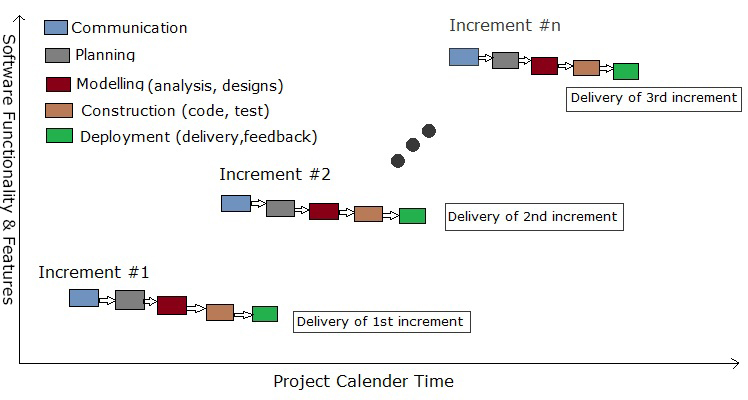
\includegraphics[width=1\linewidth]{Incremental-Development}
			\caption[Incremental Development]{Il modello incrementale consiste nella applicazione di più sequenze lineari scalate nel tempo}
			\label{fig:incremental-development}
		\end{figure}
	
		Il \textit{modello di processo incrementale} combina alcuni aspetti del modello a cascata applicati a sottoinsiemi del prodotto finale. Il modello incrementale consiste nell'applicare più sequenze lineari, scalate nel tempo. Ogni sequenza lineare produce uno "stadio" operativo del software scalato nel tempo.\\
		Il modello a processo incrementale è essenzialmente iterativo, grazie alla pianificazione della sequenza degli stadi inoltre si può controllare i rischi di natura tecnica.\\
		Ogni processo è caratterizzato da una personale \textit{milestone} che rappresenta la data di un traguardo. Ha durata pari a 1 giorno e coincide con la consegna dei documenti in vista della successiva revisione o l'approvazione di quanto fatto a monte del periodo. Nei diagrammi di pianificazione è indicata con delle linee rosse sul giorno prestabilito.
		\subsection{Scelte di alto livello}
			Completato il periodo di analisi, viene disegnata l'architettura logico-funzionale del sistema software. Vengono, cioè, effettuate le scelte di alto livello relative alla strutturazione del sistema in (macro)parti distinte (sottosistemi), definite le responsabilità di ciascun sottosistema, le modalità di dialogo (interfacce) tra i diversi sottosistemi, i dati trattati dai componenti.
			Definizione quindi delle priorità di realizzazione:
			\begin{itemize}
				\item priorità di natura funzionale (relative alle esigenze del committente);
				\item priorità di natura architetturale (ad es. se un sottosistema A necessita del sottosistema B per funzionare, B ha una priorità superiore).
			\end{itemize}
		
			
	\newpage	
	
	\rhead{Pianificazione di Progetto}
	\section{Pianificazione di Progetto}
	Il gruppo \textit{SWEg} ha deciso di suddividere lo sviluppo del progetto in cinque macro-fasi:
	\begin{enumerate}
		\item \textbf{Analisi} (AN);
		\item \textbf{Analisi Dettaglio} (AD);
		\item \textbf{Progettazione Architetturale} (PA);
		\item \textbf{Progettazione di Dettaglio e Codifica} (PDC);
		\item \textbf{Validazione e Collaudo} (VC).
	\end{enumerate}
	Ogni macro-periodo è poi stata suddivisa in attività più piccole, alle quali sono state associate una o più risorse. \\
	Per facilità di scomposizione si è scelta una semplice divisione:
	\begin{itemize}
		\item \textbf{Per capitoli}: ogni documento presenta dei capitoli prestabiliti e quindi un singolo può completare uno o più capitoli del documento;
		\item \textbf{Per azione}: a seconda di cui il singolo è specializzato ricopre un'attività inerente al suo ruolo. (Es: Esperto di produce un template, ecc...);
		\item \textbf{Verifica}: ogni documento e azione ha bisogno di verifica obbligatoria. Quindi è assegnata ai componenti in cui non vi è conflitto di interesse sulla stesura da parte del \textit{Project Manager}.
	\end{itemize} 
	La scomposizione non è segnata negli schemi.\\
	Riportiamo inoltre la \textit{work breakdown structure}\textsubscript{g} detta anche struttura di scomposizione del lavoro (traduzione letterale) o struttura analitica di progetto, si intende l'elenco di tutte le attività di un progetto. Sono usate dal \textit{Project Manager} per aiutarlo nella suddivisione e nel calcolo dei costi di ogni parte del progetto. Inoltre aiutano i componenti nella comprensione dei compiti dei ruoli e dei doveri.
	Per il glossario la tempistica di stesura è non quantificabile (n.q.) in quanto ogni componente del team dà il suo contributo durante tutta l'elaborazione de prodotto.
	
	
	\subsection{Analisi}
	\textit{\begin{center} Periodo: dal 04-11-2016 al 21-12-2016. \end{center}} 
	Questo stadio inizia con la presentazione dei capitolati d'appalto e termina con la scadenza di
	consegna della documentazione.
	\\
	Le attività nel punto di Analisi sono:
	\begin{enumerate}
		\item \textbf{Studio di Fattibilità}: vengono valutati tutti i capitolati d'appalto e viene redatto uno studio di fattibilità.
		Viene studiata la complessità delle varie proposte mediante un abbozzo di \textit{Analisi dei Requisiti v1.0.0} ad alto livello.
		La prima attività da eseguire in quanto bloccante per l'\textit{Analisi dei Requisiti v1.0.0}. Concluso lo 
		studio di fattibilità si decide quale progetto il gruppo ambisce a realizzare;
		\item \textbf{Norme di progetto}: l'\textit{Amministratore} emana le norme che il gruppo sarà obbligato a seguire
		durante le attività. Sarà poi compito dei verificatori accertare il rispetto di tali norme;
		\item \textbf{Analisi dei Requisiti v1.0.0}: viene fatta un'analisi approfondita partendo dalla base fatta durante lo Studio di Fattibilità. Questa attività continuerà fino alla data di consegna;
		\item \textbf{Piano di Progetto v1.0.0}: il responsabile del gruppo redige questo documento così da organizzare le attività del gruppo. Questa attività ha un'alta priorità;
		\item \textbf{Piano di Qualifica v1.0.0}: l'\textit{Analista} redige il Piano di Qualifica in collaborazione con l'\textit{Amministratore} ed il \textit{Responsabile di Progetto}; 
		\item \textbf{Glossario v1.0.0}: viene scritto in modo incrementale da chi redige i documenti. Contiene la spiegazione di alcuni termini utilizzati. Viene redatto in parallelo a tutti i documenti ed è aggiornato ad ogni termine che necessita di una spiegazione;
		\item \textbf{Lettera di presentazione}: documento presentato al committente che permette al gruppo di partecipare alla gara d'appalto per il capitolato.
	\end{enumerate}
	In questa macro-periodo i ruoli maggiormente coinvolti sono: \textit{Responsabile}, \textit{Amministratore}, \textit{Analista}. \\
	Per facilità di rappresentazione lo schema è riportato insieme all' \textit{Analisi in Dettaglio}.
	
	\subsection{Analisi in dettaglio}
	\textit{\begin{center} Periodo: dal 22-12-2016 al 11-01-2017 \end{center}}
	Questa sezione di progetto inizia dopo la \textit{Revisione dei Requisiti} e termina con l'inizio dell'attività di \textit{Progettazione Architetturale}.
	In questa attività sostanzialmente viene migliorata l'\textit{Analisi dei Requisiti v1.0.0}.
	\\
	I ruoli maggiormente coinvolti sono il \textit{Responsabile}, l'\textit{Amministratore} e l'\textit{Analista}. \\
	
	\begin{figure}[p]
		\centering
		\includegraphics[width=1\linewidth]{"Gantt Analisi"}
		\caption{Analisi e Analisi in Dettaglio}
		\label{fig:gantt-progettazione-architetturale}
	\end{figure}

	\begin{figure}[p]
		\centering
		\includegraphics[width=0.6\linewidth]{"WBSAnalisi"}
		\caption{Work Breakdown Structure Analisi}
		\label{fig:WBSAnalisi}
	\end{figure}

	\subsubsection{Distribuzione del lavoro}{
		\small
			{\renewcommand\arraystretch{1.1} %aumenta l'altezza di ogni riga
			\begin{tabular}{|c|l|r|c|}
				\hline
				{\textbf{Codice}}&{\textbf{Attività}}&{\textbf{Ruolo}}&{\textbf{Ore + Verifica}}\\
				\hline
				\textbf{AN1} & \textbf{Norme di Progetto} & & \textbf{8,5 + 3} \\
				
				AN1.1 & Introduzione & Amministratore & 1 \\
				
				AN1.2 & Procedure di Sviluppo & Project Manager & 1 \\
				
				AN1.3 & Documenti & Amministratore & 1,5 \\
				
				AN1.4 & Analisi dei Requisiti & Project Manager & 1 \\
				
				AN1.5 & Ruoli & Project Manager & 1 \\
				
				AN1.6 & Ambiente di Lavoro & Project Manager & 1 \\
				
				AN1.7 & Comunicazioni e Riunioni & Project Manager & 1 \\
				
				AN1.8 & Versionamento & Project Manager & 1 \\
				
				AN1.9 &	Verifica & Verificatore & 3 \\
				\hline
				\textbf{AN2} & \textbf{Piano di Qualifica} & & \textbf{11 + 3,5} \\
				
				AN2.1 & Gestione Amministrativa & Amministratore & 1,5 \\
				
				AN2.2 & Introduzione & Amministratore & 1 \\
				
				AN2.3 & Definizione degli Obbiettivi & Definizione degli Obbiettivi & 3 \\
				
				AN2.4 & Visione generale delle Strategia di Verifica & Amministratore & 3,5 \\
				
				AN2.5 & Resoconto delle Attività di Verifica & Amministratore & 2 \\
				
				AN2.6 & Verifica & Verificatore & 3,5 \\
				\hline
				\textbf{AN3} & \textbf{Piano di Progetto} & & \textbf{13 + 4} \\
				
				AN3.1 & Introduzione & Amministratore & 1 \\
				
				AN3.2 & Scadenze & Project Manager & 1 \\
				
				AN3.3 & Analisi dei Rischi & \minitab[r]{Analista \\ Project Manager} & 2,5 \\
				
				AN3.4 & Modello di Sviluppo & Project Manager & 1 \\
				
				AN3.5 & Pianificazione del Progetto & Project Manager & 2 \\
				
				AN3.6 & Preventivo & \minitab[r]{Analista \\ Project Manager} & 3 \\
				
				AN3.7 & Preventivo a Finire & Project Manager & 2 \\
				
				AN3.8 & Consultivo di Periodo & Project Manager & 0,5 \\
				
				AN3.9 & Verifica & Verificatore & 4 \\
				\hline
				\textbf{AN4} & \textbf{Studio Di Fattibilità} & & \textbf{9,5 + 3} \\
				
				AN4.1 & Capitolato C1 - API Market & Analista & 3,5 \\
				
				AN4.2 & Introduzione & Amministratore & 1 \\
				
				AN4.3 & Confronto con gli altri Capitolati & Analista & 5 \\
				
				AN4.4 & Verifica & Verificatore & 3 \\
				\hline
				\textbf{AN5} & \textbf{Analisi dei Requisiti} & & \textbf{49,5 + 16,5} \\
				
				AN5.1 & Introduzione & Amministratore & 1 \\
				
				AN5.2 & Analisi del Capitolato & Analisti & 10 \\
				
				AN5.3 & Descrizione Generale & Analista & 3 \\
				
				AN5.4 & Casi d'uso & Analisti & 20 \\
				
				AN5.5 & Grafici UML & Analisti & 15,5 \\
				
				AN5.6 & Verifica & Verificatore & 16,5 \\
				\hline
				\textbf{AN6} & \textbf{Glossario} & & \textbf{n.q. + 1} \\
				
				AN6.1 & Introduzione & Amministratore & 0.5 \\
				 
				AN6.2 & Stesura & & n.q. \\
						
				AN6.3 & Verifica & Verificatore & 1 \\
				\hline	
			\end{tabular}
		}
		\normalsize
	}
	
	\subsection{Progettazione Architetturale}
	\begin{center}\textit{Periodo: dal 25-01-2017 al 13-03-2017}\end{center}
	Questo punto termina con la pubblicazione dell'esito all'ammissione di progetto, lasciando l'attività successiva lo stato definitivo del prodotto stesso. Le attività in questo caso sono:
	\begin{enumerate}
		\item \textbf{Specifica Tecnica}: il \textit{Progettista} espone le scelte progettuali che il prodotto dovrà avere.\\
		Verranno descritti i design pattern utilizzati nella creazione del prodotto, l'architettura generale del software, i principali flussi di controllo ed il tracciamento dei requisiti;
		\item \textbf{Incremento e verifica}: tutti i documenti verranno aggiornati in base al risultato della Revisione dei Requisiti.
	\end{enumerate}
	Le figure maggiormente coinvolte sono il \textit{Responsabile}, l'\textit{Amministratore}, il \textit{Progettista}, l'\textit{Analista}
	ed il \textit{Verificatore}. \\
	
	\begin{figure}[p]
		\centering
		\includegraphics[width=1\linewidth]{"Gantt Progettazione Architetturale"}
		\caption{Progettazione Architetturale}
		\label{fig:gantt-progettazione-architetturale}
	\end{figure}

	\begin{figure}[p]
		\centering
		\includegraphics[width=0.8\linewidth]{"WBSArchitetturale"}
		\caption{Work Breakdown Structure Progettazione Architetturale}
		\label{fig:WBSArchitetturale}
	\end{figure}

	\subsubsection{Distribuzione del lavoro}{
		\small
		{\renewcommand\arraystretch{1.1} %aumenta l'altezza di ogni riga
			\begin{tabular}{|c|l|r|c|}
				\hline
				{\textbf{Codice}}&{\textbf{Attività}}&{\textbf{Ruolo}}&{\textbf{Ore + Verifica}}\\
				\hline
				\textbf{PA1} & \textbf{Norme di Progetto} & & \textbf{4 + 1.5 } \\
				
				PA1.1 & Incremento & Project Manager & 4 \\
				
				PA1.2 &	Verifica & Verificatore & 1.5 \\
				\hline
				\textbf{PA2} & \textbf{Piano di Qualifica} & & \textbf{10.5 + 3.5 } \\
				
				PA2.1 & Incremento & Amministratore & 3.75 \\
				
				PA2.2 & Pianificazione dei Test & Amministratore & 6.75 \\
				
				PA2.3 & Verifica & Verificatore & 3.5 \\
				\hline
				\textbf{PA3} & \textbf{Piano di Progetto} & & \textbf{9 + 3} \\
				
				PA3.1 & Incremento & Project Manager & 8.5 \\
				
				PA3.2 & Consultivo di Periodo & Project Manager & 0.5 \\
				
				PA3.3 & Verifica & Verificatore &  \\
				\hline
				\textbf{PA4} & \textbf{Analisi dei Requisiti (+SdF)} & & \textbf{2 + } \\
				
				PA4.1 & Incremento & Analista & 2 \\
				
				PA4.2 & Verifica & Verificatore & 3 \\
				\hline
				\textbf{PA5} & \textbf{Specifica Tecnica} & & \textbf{112.5 + 37 } \\
				
				PA5.1 & Introduzione & Amministratore & 1 \\
				
				PA5.2 & Definizione del Prodotto & Progettisti & 25 \\
				PA5.2.1 & Architettura Generale & Progettisti & 5.5 \\
				PA5.2.2 & Metodo e Formalismo & Progettisti & 19.5 \\
				
				PA5.3 & Strumenti e Tecnologie & Progettisti & 6 \\
				
				PA5.4 & Design Pattern & Progettisti & 13.5 \\
				
				PA5.5 & Descrizione Singoli Componenti & Progettisti & 21 \\
				
				PA5.6 & Stima di Fattibilità e Risorse & \minitab[r]{Progettisti \\ Analisti} & 20 \\
				
				PA5.7 & Tracciamento & & 26 \\
				PA5.7.1 & Componenti - Requisiti & \minitab[r]{Progettisti \\ Analisti} & 13 \\
				PA5.7.2 & Requisiti - Componenti & \minitab[r]{Progettisti \\ Analisti} & 13 \\
				
				PA5.8 & Verifica & Verificatore & 37 \\
				\hline
				\textbf{PA6} & \textbf{Glossario} & & \textbf{n.q. + 0.5 } \\
				
				PA6.1 & Stesura & & n.q. \\
				
				PA6.2 & Verifica & Verificatore & 0.5 \\
				\hline	
			\end{tabular}
		}
		\normalsize
	}
	
	\subsection{Progettazione di Dettaglio e Codifica}
	\textit{\begin{center} Periodo: dal 14-03-2017 al 17-04-2015 \end{center}}
	Inizia dopo la \textit{Revisione di Progetto} e termina con la consegna del prodotto alla \textit{Revisione di Qualifica}.\\
	Le attività di questo stadio sono:
	\begin{itemize}
		\item \textbf{Definizione di Prodotto}: viene definita la struttura in modo approfondito e le varie relazioni dei vari componenti del prodotto, basandosi sul documento di
		\textit{Specifica Tecnica};
		\item \textbf{Codifica}: inizia lo sviluppo del codice da parte dei programmatori, che devono seguire quanto riportato nel documento \textit{Definizione di Prodotto};
		\item \textbf{Manuale utente}: questo documento ha lo scopo di fornire delle linee guida per l'utilizzo del sistema;
		\item \textbf{Incremento e Verifica}: tutti i documenti verranno aggiornati in base al risultato della \textit{Revisione di Progettazione}.
	\end{itemize}
	I ruoli coinvolti sono il \textit{Responsabile}, l'\textit{Amministratore}, il \textit{Progettista}, il \textit{Verificatore}
	ed il \textit{Programmatore}.\\
	
	\begin{figure}[p]
		\centering
		\includegraphics[width=1\linewidth]{"Gantt Progettazione di Dettaglio"}
		\caption{Progettazione di Dettaglio e Codifica}
		\label{fig:gantt-progettazione-di-dettaglio}
	\end{figure}

	\begin{figure}[p]
		\centering
		\includegraphics[width=0.9\linewidth]{"WBSCodifica"}
		\caption{Work Breakdown Structure Progettazione di Dettaglio e Codifica}
		\label{fig:WBSCodifica}
	\end{figure}

	\subsubsection{Distribuzione del lavoro}{
		\small
		{\renewcommand\arraystretch{1.1} %aumenta l'altezza di ogni riga
			\begin{tabular}{|c|l|r|c|}
				\hline
				{\textbf{Codice}}&{\textbf{Attività}}&{\textbf{Ruolo}}&{\textbf{Ore + Verifica}}\\
				\hline
				\textbf{PD1} & \textbf{Norme di Progetto} & & \textbf{1.5 + 1} \\
				
				PD1.1 & Incremento & Project Manager & 1.5 \\
				
				PD1.2 &	Verifica & Verificatore & 1 \\
				\hline
				\textbf{PD2} & \textbf{Piano di Qualifica} & & \textbf{9 + 5} \\
				
				PD2.1 & Incremento & Amministratore & 4 \\
				
				PD2.2 & Pianificazione dei Test & Amministratore & 5 \\
				
				PD2.3 & Verifica & Verificatore & 5 \\
				\hline
				\textbf{PD3} & \textbf{Piano di Progetto} & & \textbf{3.5 + 2} \\
				
				PD3.1 & Incremento & Project Manager & 3 \\
				
				PD3.2 & Consultivo di Periodo & Project Manager & 0.5 \\
				
				PD3.3 & Verifica & Verificatore & 2 \\
				\hline
				\textbf{PD4} & \textbf{Specifica Tecnica} & & \textbf{78 + 44} \\
				
				PD4.1 & Incremento & Progettista & 6 \\
				
				PD4.2 & Definizione del Prodotto & Progettisti & 59 \\
				PD4.2.1 & Standard di Progetto & Progettisti & 29.5 \\
				PD4.2.2 & Specifica delle Componenti & Progettisti & 29.5 \\
				
				PD4.3 & Tracciamento & & 13 \\
				PD4.3.1 & Requisiti - Componenti & \minitab[r]{Progettisti \\ Analisti} & 13 \\
				
				PD4.4 & Verifica & Verificatore &  \\
				\hline
				\textbf{PD5} & \textbf{Resoconto Attività} & & \textbf{16 + 0} \\
				
				PD5.1 & Analisi Statica & Verificatori & 8 \\
				
				PD5.2 & Analisi Dinamica & Verificatori & 8 \\
				\hline
				\textbf{PD6} & \textbf{Manuale Utente} & & \textbf{15 + 8.5} \\
				
				PD6.1 & Stesura & Programmatore & 15 \\
				
				PD6.2 & Verifica & Verificatore &  \\
				\hline
				\textbf{PD7} & \textbf{Codifica} & Programmatori & \textbf{86} \\
				\hline
				\textbf{PD8} & \textbf{Glossario} & & \textbf{n.q. + 0.5 } \\
				
				PD8.1 & Stesura & & n.q. \\
				
				PD8.2 & Verifica & Verificatore & 0.5 \\
				\hline	
			\end{tabular}
		}
		\normalsize
	}
		
	
	\subsection{Validazione e Collaudo}
	\textit{\begin{center} Periodo: dal 18-04-2017 al 14-05-2015 \end{center}}
	Questa macro-sequenza riunisce tutti i test dalla più piccola quantità di software che conviene testare da sola al progetto complessivamente.\\
	Ogni esame è correlato di un \textit{Analisi Statica} e \textit{Analisi Dinamica} che coincidono in modo complementare con un periodo di progettazione e/o realizzazione.\\
	Vi è l'obbligo di utilizzo di metodi automatici per la realizzazione dei test, onde evitare errori umani . Se nel corso del progetto si è svolta una verifica passo per passo, la validazione è spontanea. \\ 
	Rappresenta l'atto conclusivo delle varie attività di verifica realizzate nei singoli processi del ciclo di vita.
	Le attività sono:
	\begin{enumerate}
		\item \textbf{Test di Unità};
		\item \textbf{Test di Integrazione};
		\item \textbf{Test di Sistema};
		\item \textbf{Collaudo};
		\item \textbf{Validazione}: controllo generico di tutti i documenti.
	\end{enumerate}
	I ruoli coinvolti sono il \textit{Responsabile}, l'\textit{Amministratore}, il \textit{Progettista} ed il \textit{Verificatore}.
	
	\begin{figure}[p]
		\centering
		\includegraphics[width=1\linewidth]{"Gantt Validazione e Collaudo"}
		\caption{Validazione e Collaudo}
		\label{fig:gantt-validazione-e-collaudo}
	\end{figure}

	\begin{figure}[p]
		\centering
		\includegraphics[width=1\linewidth]{"WBSValidazione"}
		\caption{Work Breakdown Structure Validazione e Collaudo}
		\label{fig:WBSValidazione}
	\end{figure}

	\subsubsection{Distribuzione del lavoro}{
		\small
		{\renewcommand\arraystretch{1.1} %aumenta l'altezza di ogni riga
			\begin{tabular}{|c|l|r|c|}
				\hline
				{\textbf{Codice}}&{\textbf{Attività}}&{\textbf{Ruolo}}&{\textbf{Ore + Verifica}}\\
				\hline
				\textbf{VA1} & \textbf{Norme di Progetto} & & \textbf{1.5 + 3 } \\
				
				VA1.1 & Incremento & Project Manager & 1.5 \\
				
				VA1.2 &	Verifica & Verificatore & 3 \\
				\hline
				\textbf{PD2} & \textbf{Piano di Qualifica} & & \textbf{7 + 5 } \\
				
				VA2.1 & Incremento & Amministratore & 7 \\
				
				VA2.2 & Verifica & Verificatore & 5 \\
				\hline
				\textbf{VA3} & \textbf{Piano di Progetto} & & \textbf{3 + 4 } \\
				
				VA3.1 & Incremento & Project Manager & 2.5 \\
				
				VA3.2 & Consultivo di Periodo & Project Manager & 0.5 \\
				
				VA3.3 & Verifica & Verificatore & 4 \\
				\hline
				\textbf{VA4} & \textbf{Specifica Tecnica} & & \textbf{5.5 + 5 } \\
				
				VA4.1 & Incremento & Progettista & 2.75 \\
				
				VA4.2 & Definizione del Prodotto & Progettisti & 2,75 \\
				VA4.2.1 & Incremento & Progettisti & 2,75 \\
				
				VA4.3 & Verifica & Verificatore & 5 \\
				\hline
				\textbf{VA5} & \textbf{Glossario} & & \textbf{n.q. + 1} \\
				
				VA5.1 & Stesura & & n.q. \\
				
				VA5.2 & Verifica & Verificatore & 1 \\
				\hline
				\textbf{VA6} & \textbf{Manuale Utente} & & \textbf{3 + 4} \\
				
				VA6.1 & Incremento & Programmatore & 3 \\
				
				VA6.2 & Verifica & Verificatore & 4 \\
				\hline
				\textbf{VA7} & \textbf{Collaudo} & \minitab[l]{ Programmatore \\ Verificatore } & \textbf{5} \\
				\hline
			\end{tabular}
		}
		\normalsize
	}
	\newpage
	
	\rhead{Preventivo}
	\section{Preventivo}
	Qui vengono presentate le ore preventivate di impiego per i vari ruoli coinvolti.\\
	Si ricorda che il periodo di \textit{Analisi dei Requisiti} e \textit{Analisi Dettaglio} non sono a carico del committente e quindi non saranno considerate nel calcolo delle ore totali da retribuire. \\
	Costi e sigle delle tabelle fanno riferimento al capitolo \textit{Ruoli} del documento: \textit{Norme di Progetto v2.0.0}.
	
	\subsection{Analisi}
	Nel periodo di analisi non vi sono ore di \textit{Codifica}, eseguite dal \textit{Programmatore}, e di \textit{Progettazione}, eseguite dal \textit{Progettista}. Questo perché Analisi e Progettazione non sono mai simultaneamente attive. \\
	Durante il periodo di Analisi le ore tra i ruoli sono state divise nel modo seguente: \\
	
	{\renewcommand\arraystretch{1.2} %aumenta l'altezza di ogni riga
		\small
		\begin{tabular}{|c|c|c|c|c|c|c|c|}
			\hline 
			\textbf{Nome} & \multicolumn{6}{c|}{\textbf{Ore e Costo per Ruolo}} & \textbf{Totale} \\ 
			& \textbf{PM} & \textbf{AM} & \textbf{AN} & \textbf{PL} & \textbf{PR} & \textbf{VE} & \textbf{} \\ 
			\hline
			Sebastiano Marchesini & 8x30 & 9x20 & 4x25 & & & & 520,00 \\ 
			\hline 
			Gianluca Crivellaro & & & 18x25 & & & 3x15 & 495,00 \\ 
			\hline 
			Pietro Lonardi & & & 13x25 & & & 7x15 & 430,00 \\ 
			\hline 
			Alberto Gelmi & & & 8x25 & & & 7x15 & 305,00 \\ 
			\hline 
			Piergiorgio Danieli & 5x30 & 5x20 & & & & 12x15 & 430,00 \\ 
			\hline
			\textbf{Ore Totali per ruolo} & 13 & 14 & 43 & 0 & 0 & 29 & 99 \\  
			\textbf{Prezzo Totale per ruolo}&\euro 390,00&\euro 280,00&\euro  1.075,00&\euro 0,00&\euro 0,00&\euro 435,00& \textit{\euro 2.180,00} \\
			\hline  
	\end{tabular}} 
	
	\subsection{Analisi Dettaglio}
	Analisi Dettaglio concentra tutto il team sul documento di \textit{Analisi dei Requisiti v1.0.0}. Ognuno pone la sua attenzione su un particolare argomento del progetto, si analizza, guidati dal \textit{Project Manager}. L'\textit{Amministratore} è a capo delle revisioni . Non vi sono altri compiti da svolgere in questo stadio, quindi non vi sono altre ore rendicontate.\\
	Nel periodo che riguarda l'Analisi Dettaglio, le ore tra i ruoli sono state divise come segue:\\
	
	{\renewcommand\arraystretch{1.2} %aumenta l'altezza di ogni riga
		\small
		\begin{tabular}{|c|c|c|c|c|c|c|c|}
			\hline 
			\textbf{Nome} & \multicolumn{6}{c|}{\textbf{Ore e Costo per Ruolo}} & \textbf{Totale} \\ 
			& \textbf{PM} & \textbf{AM} & \textbf{AN} & \textbf{PL} & \textbf{PR} & \textbf{VE} & \textbf{} \\ 
			\hline
			Sebastiano Marchesini & & & 1x25 & & & 3x15 & 70,00 \\ 
			\hline 
			Gianluca Crivellaro & 1x30 & & 4x25 & & & 1x15 & 145,00 \\ 
			\hline 
			Pietro Lonardi & & 1x20 & 3x25 & & & 2x15 & 125,00 \\ 
			\hline 
			Alberto Gelmi & & & 3x25 & & & 1x15 & 90,00 \\ 
			\hline 
			Piergiorgio Danieli & & & 2x25 & & & 3x15 & 95,00 \\ 
			\hline
			\hline
			\textbf{Ore Totali per ruolo} & 1 & 1 & 13 & 0 & 0 & 10 & 25 \\  
			\textbf{Prezzo Totale per ruolo}&\euro 30,00&\euro 20,00&\euro 325,00&\euro 0,00&\euro 0,00&\euro 150,00& \textit{\euro 525,00} \\
			\hline  
	\end{tabular}} 

	\begin{figure}[p]
		\centering
		\includegraphics[width=0.7\linewidth]{"CiambellaAnalisi"}
		\caption{Percentuale Ruoli Analisi e Analisi in Dettaglio}
		\label{fig:ciambella-progettazione-analisi}
	\end{figure} 
	
	
	\subsection{Progettazione Architetturale}
	Anche in questo periodo viene meno un ruolo del team che può svolgere solo una funzione: quella del \textit{Programmatore}. Trovare soluzioni alle analisi rilevate non è suo compito ma solo di tradurre in linguaggio di programmazione le decisioni del \textit{Progettista}.\\
	Nel periodo riguardante la Progettazione Architetturale le ore tra i ruoli sono stati divisi nel seguente modo:\\
	
	{\renewcommand\arraystretch{1.2} %aumenta l'altezza di ogni riga
		\small
		\begin{tabular}{|c|c|c|c|c|c|c|c|}
			\hline 
			\textbf{Nome} & \multicolumn{6}{c|}{\textbf{Ore e Costo per Ruolo}} & \textbf{Totale} \\ 
			& \textbf{PM} & \textbf{AM} & \textbf{AN} & \textbf{PL} & \textbf{PR} & \textbf{VE} & \textbf{} \\ 
			\hline 
			Sebastiano Marchesini & 2x30 & & 5x25 & 13x22 & & 12x15 & 651,00 \\ 
			\hline 
			Gianluca Crivellaro & 8x30 & 3x20 & 7x25 & 19x22 & & 8x15 & 1.013,00 \\ 
			\hline 
			Pietro Lonardi & & 8x20 & & 11x22 & & 11x15 & 467,00 \\ 
			\hline 
			Alberto Gelmi & 3x30 & & 4x25 & 27x22 & & 3x15 & 829,00 \\ 
			\hline 
			Piergiorgio Danieli & & & 2x25 & 14x22 & & 12x15 & 538,00 \\ 
			\hline
			\hline
			\textbf{Ore Totali per ruolo} & 13 & 11 & 18 & 84 & 0 & 46 & 172 \\  
			\textbf{Prezzo Totale per ruolo}&\euro 390,00&\euro 220,00&\euro 450,00&\euro 1.848,00&\euro 0,00&\euro 690,00& \textit{\euro 3.598,00} \\
			\hline 
	\end{tabular}} 

	\begin{figure}[p]
		\centering
		\includegraphics[width=0.7\linewidth]{"CiambellaProgettazione"}
		\caption{Percentuale Ruoli Progettazione Architetturale}
		\label{fig:ciambella-progettazione-architetturale}
	\end{figure} 

	
	\subsection{Progettazione di Dettaglio e Codifica}
	Oramai tutta l'analisi è completata e quindi il ruolo dell'\textit{Analista} è praticamente sostituito dal \textit{Progettista}. Inoltre la codifica apre le porte alla programmazione effettiva e quindi al ruolo di \textit{Programmatore}.\\
	Durante la Progettazione di Dettaglio e Codifica le ore tra i ruoli sono stai divisi come segue:
	\\
	
	{\renewcommand\arraystretch{1.2} %aumenta l'altezza di ogni riga
		\small
		\begin{tabular}{|c|c|c|c|c|c|c|c|}
			\hline 
			\textbf{Nome} & \multicolumn{6}{c|}{\textbf{Ore e Costo per Ruolo}} & \textbf{Totale} \\ 
			& \textbf{PM} & \textbf{AM} & \textbf{AN} & \textbf{PL} & \textbf{PR} & \textbf{VE} & \textbf{} \\ 
			\hline
			Sebastiano Marchesini & 2x30 & & & 22x22 & 29x15 & 9x15 & 1.039,00 \\ 
			\hline 
			Gianluca Crivellaro & & 5x20 & & 18x22 & 18x15 & 12x15 & 946,00 \\ 
			\hline 
			Pietro Lonardi & 3x30 & 3x20 & & 17x22 & 15x15 & 28x15 & 1.169,00 \\ 
			\hline 
			Alberto Gelmi & & & 2x25 & 9x22 & 32x15 & 16x15 & 968,00 \\ 
			\hline 
			Piergiorgio Danieli & & 4x20 & 2x25 & 20x22 & 22x15 & 12x15 & 1.080,00 \\ 
			\hline
			\hline
			\textbf{Ore Totali per ruolo} & 5 & 12 & 4 & 86 & 104 & 82 & 293 \\  
			\textbf{Prezzo Totale per ruolo}&\euro 150,00&\euro 240,00&\euro 100,00&\euro 1.898,00&\euro 1.665,00&\euro 1.155,00& \textit{\euro 5.202,00} \\
			\hline  
	\end{tabular}} 

	\begin{figure}[p]
		\centering
		\includegraphics[width=0.7\linewidth]{"CiambellaCodifica"}
		\caption{Percentuale Ruoli Progettazione in Dettaglio e Codifica}
		\label{fig:ciambella-progettazione-dettaglio-codifica}
	\end{figure} 

	
	\subsection{Validazione e Collaudo}
	Nel periodo di Validazione e Collaudo le ore tra i ruoli sono state divise nel seguente modo:
	\\
	
	{\renewcommand\arraystretch{1.2} %aumenta l'altezza di ogni riga
		\small
		\begin{tabular}{|c|c|c|c|c|c|c|c|}
			\hline 
			\textbf{Nome} & \multicolumn{6}{c|}{\textbf{Ore e Costo per Ruolo}} & \textbf{Totale} \\ 
			& \textbf{PM} & \textbf{AM} & \textbf{AN} & \textbf{PL} & \textbf{PR} & \textbf{VE} & \textbf{} \\ 
			\hline
			Sebastiano Marchesini & 4x30 & 2x20 & & & 1x15 & 6x15 & 265,00 \\ 
			\hline 
			Gianluca Crivellaro & & 1x20 & & & & 6x15 & 110,00 \\ 
			\hline 
			Pietro Lonardi & & 3x20 & & 1x22 & 2x15 & 2x15 & 142,00 \\ 
			\hline 
			Alberto Gelmi & & 2x20 & & 2x22 & 3x15 & 2x15 & 159,00 \\ 
			\hline 
			Piergiorgio Danieli & 1x30 & & & & 2x15 & 12x15 & 240,00 \\ 
			\hline
			\hline
			\textbf{Ore Totali per ruolo} & 5 & 8 & 0 & 3 & 8 & 30 & 54 \\  
			\textbf{Prezzo Totale per ruolo}&\euro 150,00&\euro  160,00&\euro 0,00&\euro 66,00&\euro 120,00&\euro 420,00& \textit{\euro 916,00} \\  
			\hline
	\end{tabular}}

	\begin{figure}[p]
		\centering
		\includegraphics[width=0.7\linewidth]{"CiambellaValidazioneCollaudo"}
		\caption{Percentuale Ruoli Validazione e Collaudo}
		\label{fig:ciambella-validazione-collaudo}
	\end{figure} 


	
	\subsection{Riepilogo}
	\subsubsection{Ore totali}
	Le ore totali previste per la realizzazione dell'intero progetto, comprese le ore di precedenti alla firma del contratto, sono le seguenti: \\
	
	{\renewcommand\arraystretch{1.2} %aumenta l'altezza di ogni riga
		\begin{tabular}{|c|c|c|c|c|c|c|c|}
			\hline 
			\textbf{Nome} & \multicolumn{6}{c|}{\textbf{Ore per Ruolo Totali}} & \textbf{Ore Totali} \\ 
			& \textbf{PM} & \textbf{AM} & \textbf{AN} & \textbf{PL} & \textbf{PR} & \textbf{VE} & \\ 
			\hline
			Sebastiano Marchesini	& 16 & 12 & 10 & 35 & 22 & 35 & 130 \\ 
			\hline 
			Gianluca Crivellaro 	& 9 & 9 & 33 & 37 & 18 & 29 & 135 \\ 
			\hline 
			Pietro Lonardi 			& 3 & 14 & 13 & 29 & 17 & 48 & 124 \\ 
			\hline 
			Alberto Gelmi 			& 3 & 2 & 14 & 38 & 31 & 32 & 120 \\ 
			\hline 
			Piergiorgio Danieli 	& 6 & 9 & 4 & 34 & 24 & 48 & 125 \\ 
			\hline 
			\multicolumn{7}{r|}{TOTALE :} & 634 \\ 
	\end{tabular}}

	\subsubsection{Ore rendicontate}
	Tolto il periodo precedente alla firma del contrattato, l'impegno di ogni singolo si tiene sotto il tetto massimo delle 105 ore ciascuno e sono così distribuite secondo i ruoli :\\
	
	{\renewcommand\arraystretch{1.2} %aumenta l'altezza di ogni riga
		\begin{tabular}{|c|c|c|c|c|c|c|c|}
			\hline 
			\textbf{Nome} & \multicolumn{6}{c|}{\textbf{Ore per Ruolo Totali}} & \textbf{Ore Totali} \\ 
			& \textbf{PM} & \textbf{AM} & \textbf{AN} & \textbf{PL} & \textbf{PR} & \textbf{VE} & \\ 
			\hline
			Sebastiano Marchesini	& 8 & 2 & 5 & 35 & 22 & 30 & 102 \\ 
			\hline 
			Gianluca Crivellaro 	& 8 & 9 & 7 & 37 & 18 & 26 & 105 \\ 
			\hline 
			Pietro Lonardi 			& 3 & 14 & 0 & 29 & 17 & 41 & 104 \\ 
			\hline 
			Alberto Gelmi 			& 3 & 2 & 6 & 38 & 31 & 25 & 105 \\ 
			\hline 
			Piergiorgio Danieli 	& 1 & 4 & 4 & 34 & 24 & 36 & 103 \\ 
			\hline 
			Ore Totale per Ruolo & 23 & 31 & 22 & 173 & 112 & 158 & 634 \\ 
	\end{tabular}}

	Tale progettazione ha portato al seguente grafico percentuale di proporzione dei ruoli:
	
	\begin{figure}[p]
		\centering
		\includegraphics[width=0.7\linewidth]{"GraficoTortaRuoliFinale"}
		\caption{Percentuale Ore Ruoli Totale}
		\label{fig:percentuale-ore-ruoli-totale}
	\end{figure} 
	
	\newpage
	
	\rhead{Consuntivo di Periodo}
	\section{Consuntivo di Periodo}
		Riepiloga i risultati di un dato periodo di attività e verrà aggiornato nel corso del progetto per dare una rendiconto preciso ed effettivo del lavoro svolto. \\
		\subsection{Analisi e Analisi Dettaglio}{
	
		{\renewcommand\arraystretch{1.2}  %aumenta l'altezza di ogni riga
			\begin{tabular}{|c|c|c|c|c|c|c|c|}
				\hline 
				\textbf{Nome} & \multicolumn{6}{c|}{\textbf{Ore Effettive per Ruolo}} & \textbf{Ore Totali} \\ 
				& \textbf{PM} & \textbf{AM} & \textbf{AN} & \textbf{PL} & \textbf{PR} & \textbf{VE} & \\ 
				\hline
				Sebastiano Marchesini & 8 & 10(+1) & 5 &  &  & 4(+1) & 27(+2) \\ 
				\hline 
				Gianluca Crivellaro & 1 &  & 24(+2) &  &  & 3 & 28(+2) \\ 
				\hline 
				Pietro Lonardi &  & 1 & 6 &  &  & 9(+2) & 17(+2) \\ 
				\hline 
				Alberto Gelmi &  &  & 9(-2) &  &  & 8 & 17(-2) \\ 
				\hline 
				Piergiorgio Danieli & 5 & 5 & 2 &  &  & 5 & 17(+0) \\ 
				\hline 
				\multicolumn{7}{r|}{TOTALE  :} & 106(+4) \\ 
		\end{tabular}} 
		
		\begin{figure}[p]
			\centering
			\includegraphics[width=0.7\linewidth]{"ConsultivoAnalisi"}
			\caption{Grafico Consultivo di Analisi e Analisi Dettaglio}
			\label{fig:consultivo-analisi}
		\end{figure} 
	
	Si è notato che c'è voluto più tempo del previsto sia nella verifica (fatti su più livelli) sia nell'amministrazione dei documenti. Gianluca si è impegnato molto nella ricerca dei requisiti e nella stesura degli stessi, più di Alberto che causa impegni di studio ha ceduto alcuni compiti. In generale è soddisfacente l'uso delle ore totali progettate per tale periodo.	\\
	Tale variante non va a impattare sul preventivo a finire in quanto l'analisi e l'analisi specifica non è un costo effettivo che ricade sul cliente finale.
	}
		

	
	
	
	\newpage
	
	\rhead{Preventivo a Finire}
	\section{Preventivo a Finire}
	Il preventivo finale va a sommare tutte i costi ad ora organizzati. Si tiene conto del massimo impegno e della qualità scelta negli standard proposti. \\
	Non vengono tenute in considerazione:
	\begin{itemize}
		\item manutenzione e preparazione dell'hardware;
		\item attività di auto-formazione per quanto concerne la strumentazione e le specifiche;
		\item le ore di \textit{Analisi} e \textit{Analisi in Dettaglio} precedenti alla \textit{Revisione dei Requisiti};
		\item correzioni alle inadempienze gravi segnalate nella revisione.
	\end{itemize}
	\subsubsection{Tabella preventiva per Ruolo}
	\begin{center}
	{\renewcommand\arraystretch{1.2} %aumenta l'altezza di ogni riga
		\begin{tabular}{|c|c|c|}
			\hline 
			\textbf{Ruolo} & \textbf{Costo orario} & \textbf{Costo Effettivo} \\ 
			\hline 
			\textbf{Responsabile Progetto} & \euro 30,00 & \euro 690,00 \\ 
			\hline 
			\textbf{Amministratore} & \euro 20,00 & \euro 620,00 \\ 
			\hline 
			\textbf{Analista} & \euro 25,00 & \euro 550,00 \\ 
			\hline 
			\textbf{Progettista} & \euro 22,00 & \euro 3.806,00 \\ 
			\hline 
			\textbf{Programmatore} & \euro 15,00 & \euro 1.785,00 \\ 
			\hline 
			\textbf{Verificatore} & \euro 15,00 & \euro 2.265,00 \\ 
			\hline 
			\multicolumn{2}{r|}{TOTALE :} & \textit{\euro 9.716,00 } \\ 
		\end{tabular}
	} 
	\vspace{0.7cm}
	\begin{figure}[p]
		\centering
		\includegraphics[width=1\linewidth]{"TortaIncisioneCosti"}
		\caption{Percentuale di Incidenza del Costo di ogni Ruolo}
		\label{fig:torta-incisione-costi}
	\end{figure}
		
	\end{center}

	\subsubsection{Tabella preventiva per periodo a finire}
	\begin{center}
	{\renewcommand\arraystretch{1.2} %aumenta l'altezza di ogni riga
		\begin{tabular}{|c|c|c|}
			\hline 
			& \textbf{Costo} & \textbf{Costo Effettivo} \\ 
			\hline 
			\textbf{Analisi} & \euro 2180,00 & \euro 00,00 \\ 
			\hline 
			\textbf{Analisi Specifica} & \euro 525,00 & \euro 00,00 \\ 
			\hline 
			\textbf{Progettazione} & \euro 3.598,00 & \euro 3.598,00 \\ 
			\hline 
			\textbf{Progettazione in Dettaglio e Codifica} & \euro 5.202,00 & \euro 5.202,00 \\ 
			\hline 
			\textbf{Validazine e Collaudo} & \euro 916,00 & \euro 916,00 \\ 
			\hline 
			\multicolumn{2}{r|}{TOTALE :} & \textit{\euro 9.716,00 } \\ 
		\end{tabular}
	} 
	\vspace{0.5cm}
	\end{center}
	
	In seguito riporteremo i danni economici che vi sono riportati confrontando il preventivo con l'effettivo consuntivo di periodo.
	
\end{document}